\subsubsection{Какова неравновесная концентрация неосновных носителей заряда на границе p и n?}
\textit{Здесь должны быть формулы относительно распределения электростатического потенциала, но они далее}

Выведем длины pn-перехода. Для этого воспользуемся уравнением Пуассона. Из предположения ступенчатости перехода следует, что $\lambda_p = - q N_a; \lambda_n = q N_d$, следовательно:
\begin{equation}
E_p = -  \frac{q N_a}{\varepsilon \varepsilon_0} (x + l_p)
\end{equation}
\begin{equation}
E_n = -  \frac{q N_d}{\varepsilon \varepsilon_0} (l_n - x)
\end{equation}
Домножая обе части уравнения на расстояние, получаем:
\begin{equation}
\phi_p - \phi_{Ep} =  -  \frac{q N_a}{2 \varepsilon \varepsilon_0} (x + l_p)^2
\end{equation}
\begin{equation}
\phi_p - \phi_{En} =  -  \frac{q N_d}{2 \varepsilon \varepsilon_0} (x - l_p)^2
\end{equation}
Тогда ширина pn-перехода равна $l_0 = l_p + l_n$:
\begin{equation}
l_0  = \sqrt{\frac{2 \varepsilon \varepsilon_0 \Delta \phi_0}{q} (\frac{1}{N_d}+ \frac{1}{N_a})}
\end{equation}
Для резко асимметричного перехода с условием $N_a >> N_d$ получаем:
\label{sec:pn_length}
\begin{equation}
l_0  = \sqrt{\frac{2 \varepsilon \varepsilon_0 \Delta \phi_0}{q N_d} }
\end{equation}
\textbf{С симметричным pn-переходом}\\
Теперь рассмотрим np-переход с приложенной к нему разностью потенциалов $U$.
При этом потенциальный барьер должен измениться. Из физических соображений  известно, что в зоне перехода практически отсутствуют свободные носители заряда, следовательно, все приложенное напряжение падает на нем.


\begin{center}
	\begin{figure}[h!]
		\center{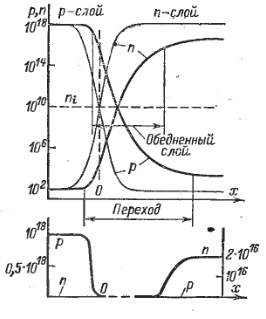
\includegraphics[scale=0.9]{pn-conc.png}}
		\caption{Плотность неосновных носителей в pn-переходе}	
		\label{pic:pn-conc}
	\end{figure}
\end{center}


Если напряжение приложено плюсом к p-слою, то такое включение называется прямым, высота потенциального барьера падает. $\Delta \phi  = \Delta \phi_0 - U$.
Иначе, высота барьера увеличивается, и, как следствие, увеличивается ширина перехода:
\begin{equation}
l = \sqrt{\frac{2 \varepsilon \varepsilon_0 ( \Delta \phi_0 - U)}{q N_d} } = l_0 \sqrt{\frac{\Delta \phi_0 -U}{\Delta \phi_0}}
\end{equation} 
При $U >> \Delta \phi_0$ 
\begin{equation}
l \approx l_0 \sqrt{\frac{|U|}{\Delta \phi_0}}
\end{equation}

Теперь выразим концентрации неосновных носителей заряда, зная новую контактную разность, концентрацию основных носителей и формулу \ref{eq:main2side_ratio}:
\begin{equation}
\Delta\varphi_0 = \varphi_Tln\frac{n_{n_0}}{n_{p_0}} = \varphi_Tln\frac{p_{p_0}}{p_{n_0}}
\end{equation}
Получаем:
\begin{equation}
p_n = p_{p0} e^{- \frac{\Delta \phi }{\phi_t}} = (p_{p0} e^{- \frac{\Delta \phi_0 }{\phi_t}}) e^{\frac{U}{\phi_t}} = 
p_{n0} e^{\frac{U}{\phi_t}}
\end{equation}
\begin{equation}
n_p = n_{n0} e^{- \frac{\Delta \phi }{\phi_t}} = (n_{n0} e^{- \frac{\Delta \phi_0 }{\phi_t}}) e^{\frac{U}{\phi_t}} = 
n_{p0} e^{\frac{U}{\phi_t}}
\end{equation}
Таким образом, при приложении прямого напряжения концентрация неосновных зарядов экспоненциально возрастает.\\
Таким образом, избыточная концентрация на границе pn-перехода:
\begin{equation}
\Delta p_n = p_{n0} (e^{\frac{U}{\phi_t}}-1)
\end{equation}
\begin{equation}
\Delta n_p = n_{p0} (e^{\frac{U}{\phi_t}}-1)
\end{equation}

\begin{center}
	\begin{figure}[h!]
		\center{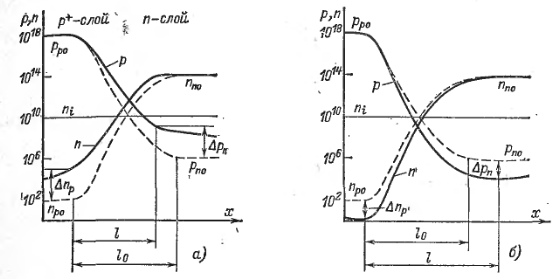
\includegraphics[scale=0.9]{np-conc_U.png}}
		\caption{Концентрация неосновных носителей заряда при обратном и прямом смещениях}	
		\label{pic:pn-conc_U}
	\end{figure}
\end{center}



Отсюда можно получить соотношение между избыточной концентрацией и концентрацией основных носителей заряда:
\begin{equation}
\frac{\Delta p_n}{\Delta n_p} = \frac{p_{p0}}{n_{n0}}
\end{equation}
Из данного соотношения следует, что при несимметричном pn-переходе (когда один из контактов сильно легирован, а другой - нет) инжекция имеет односторонний характер. Заряды инжектируются в основном из низкоомного (сильно легированного) в высокоомный (слабо легированный) слой. Инжектирующий слой тогда называют эмиттером, а другой - базой. Высота потенциального барьера, однако, в этом случае не меняется и определяется обыкновенными формулами, как и концентрация избыточных неосновных носителей заряда.



\pagebreak
